% -*- root: ../main.tex -*-
\chapter{Analisi dello spazio del problema}

Inizialmente l'esperto del dominio è stato contattato per un'intervista preliminare (sotto riportata).
La sessione si è svolta in via telematica ed ha avuto lo scopo di prendere familiarità con l'ambito di lavoro e individuare i requisiti del software ad esso collegato. 
Nel colloquio il problema è emerso chiaramente e la soluzione software è stata individuata in maniera univoca.
In seguito sono stati definiti incontri periodici con il committente per la valutazione del progresso e i feedback sui deliverables di ogni sprint.

	\section{Intervista con il committente}
    
    Sono uno studente di Ingegneria e Scienze Informatiche dell'Università di Bologna presso la sede di Cesena. In questi anni ho dovuto studiare e ripassare la teoria per molti esami e ho trovato utile porre a me stesso delle domande alle quali dover rispondere, così da verificare la conoscenza della materia.
    In particolare, dopo aver acquisito una discreta quantità di nozioni, ho riscontrato la necessità di rivedere, in maniera generale, se riuscissi a ricordare i concetti principali per ogni topic dell'esame in questione.
    Per questo motivo, sarebbe utile poter avere a disposizione uno strumento che permetta di rendere più stimolante il ripasso pre esame. Ad esempio, vorrei non dover più scrivere su un foglio le domande e le relative risposte corrette e sbagliate. In più, vorrei poterle integrare con quelle dei miei compagni e viceversa, in modo da coprire il più possibile tutti gli argomenti di un esame. Vorrei anche potermi esercitare sulle domande che sbaglio più spesso, per migliorare le lacune. Trovo utile poter ripassare più materie contemporaneamente nei periodi di sessione, in cui ho più esami nella stessa settimana. Inoltre poter rispondere a più domande possibili nel minor tempo possibile, così da essere sicuro di riuscire a rispondere velocemente durante gli orali.
    
    
    \begin{QandA}
        \item Abbiamo pensato che il modo più divertente per poter studiare e ripassare potrebbe essere quello di fare un gioco a quiz, dove viene posta una domanda e quattro possibili risposte. Potrebbe essere utile?
            \begin{answered}
            Sarebbe molto interessante, così non mi annoierei. Metterei un'unica risposta corretta e le altre tre sbagliate. Ogni volta che ripasso una materia in particolare, le domande sono sempre le stesse? Perché a me piacerebbe rispondere correttamente attraverso il ragionamento, non solo ricordandomi a memoria la risposta data in precedenza.
            \end{answered}
        \item Per quanto riguarda il numero di domande per ogni argomento, abbiamo pensato di inserirne una quantità tale da avere sempre un ricambio adeguato ed evitare il ricircolo delle stesse. Inoltre anche le risposte saranno un numero superiore alle quattro visibili per ogni domanda.
        Quali modalità di gioco vorresti avere a disposizione?
            \begin{answered}
            Mi piacerebbe poter scegliere se rispondere a domande di uno specifico corso o di più corsi durante lo stesso quiz.
            \end{answered}
        \item Riguardo al tempo disponibile per rispondere, preferisce avere un tempo limite per ogni singolo quesito o per l'intera sessione di gioco?
            \begin{answered}
            Sicuramente vorrei avere un tempo limitato ad ogni domanda, per non incorrere nella tentazione di barare. Qualora fosse possibile avere anche una modalità di gioco con un tempo limite globale sarebbe molto divertente.
            \end{answered}
        \item Invece quali schermate di gioco vorresti visualizzare?
            \begin{answered}
            Dal menu principale vorrei poter scegliere le varie modalità di gioco, poter aggiungere ed esportare le domande e le risposte dei corsi e visualizzare le statistiche sulle partite effettuate in precedenza. Invece a fine partita vorrei visualizzare un riepilogo di tutte le domande presenti nel quiz appena concluso ed eventualmente, in caso di risposta errata, visualizzare la risposta corretta.
            \end{answered}
    \end{QandA}

    \newpage
    
    \section{Ubiquitous Language}
    Per chiarire il gergo usato tra il committente e gli sviluppatori è risultato essenziale adottare dei significati condivisi per i termini maggiormente usati. Ciò ha aiutato notevolmente anche la comunicazione tra gli sviluppatori stessi per non incorrere in malintesi.
    %TABELLA UBIQUITOUS LANGUAGE
    \begin{figure}[ht]
        \centering
        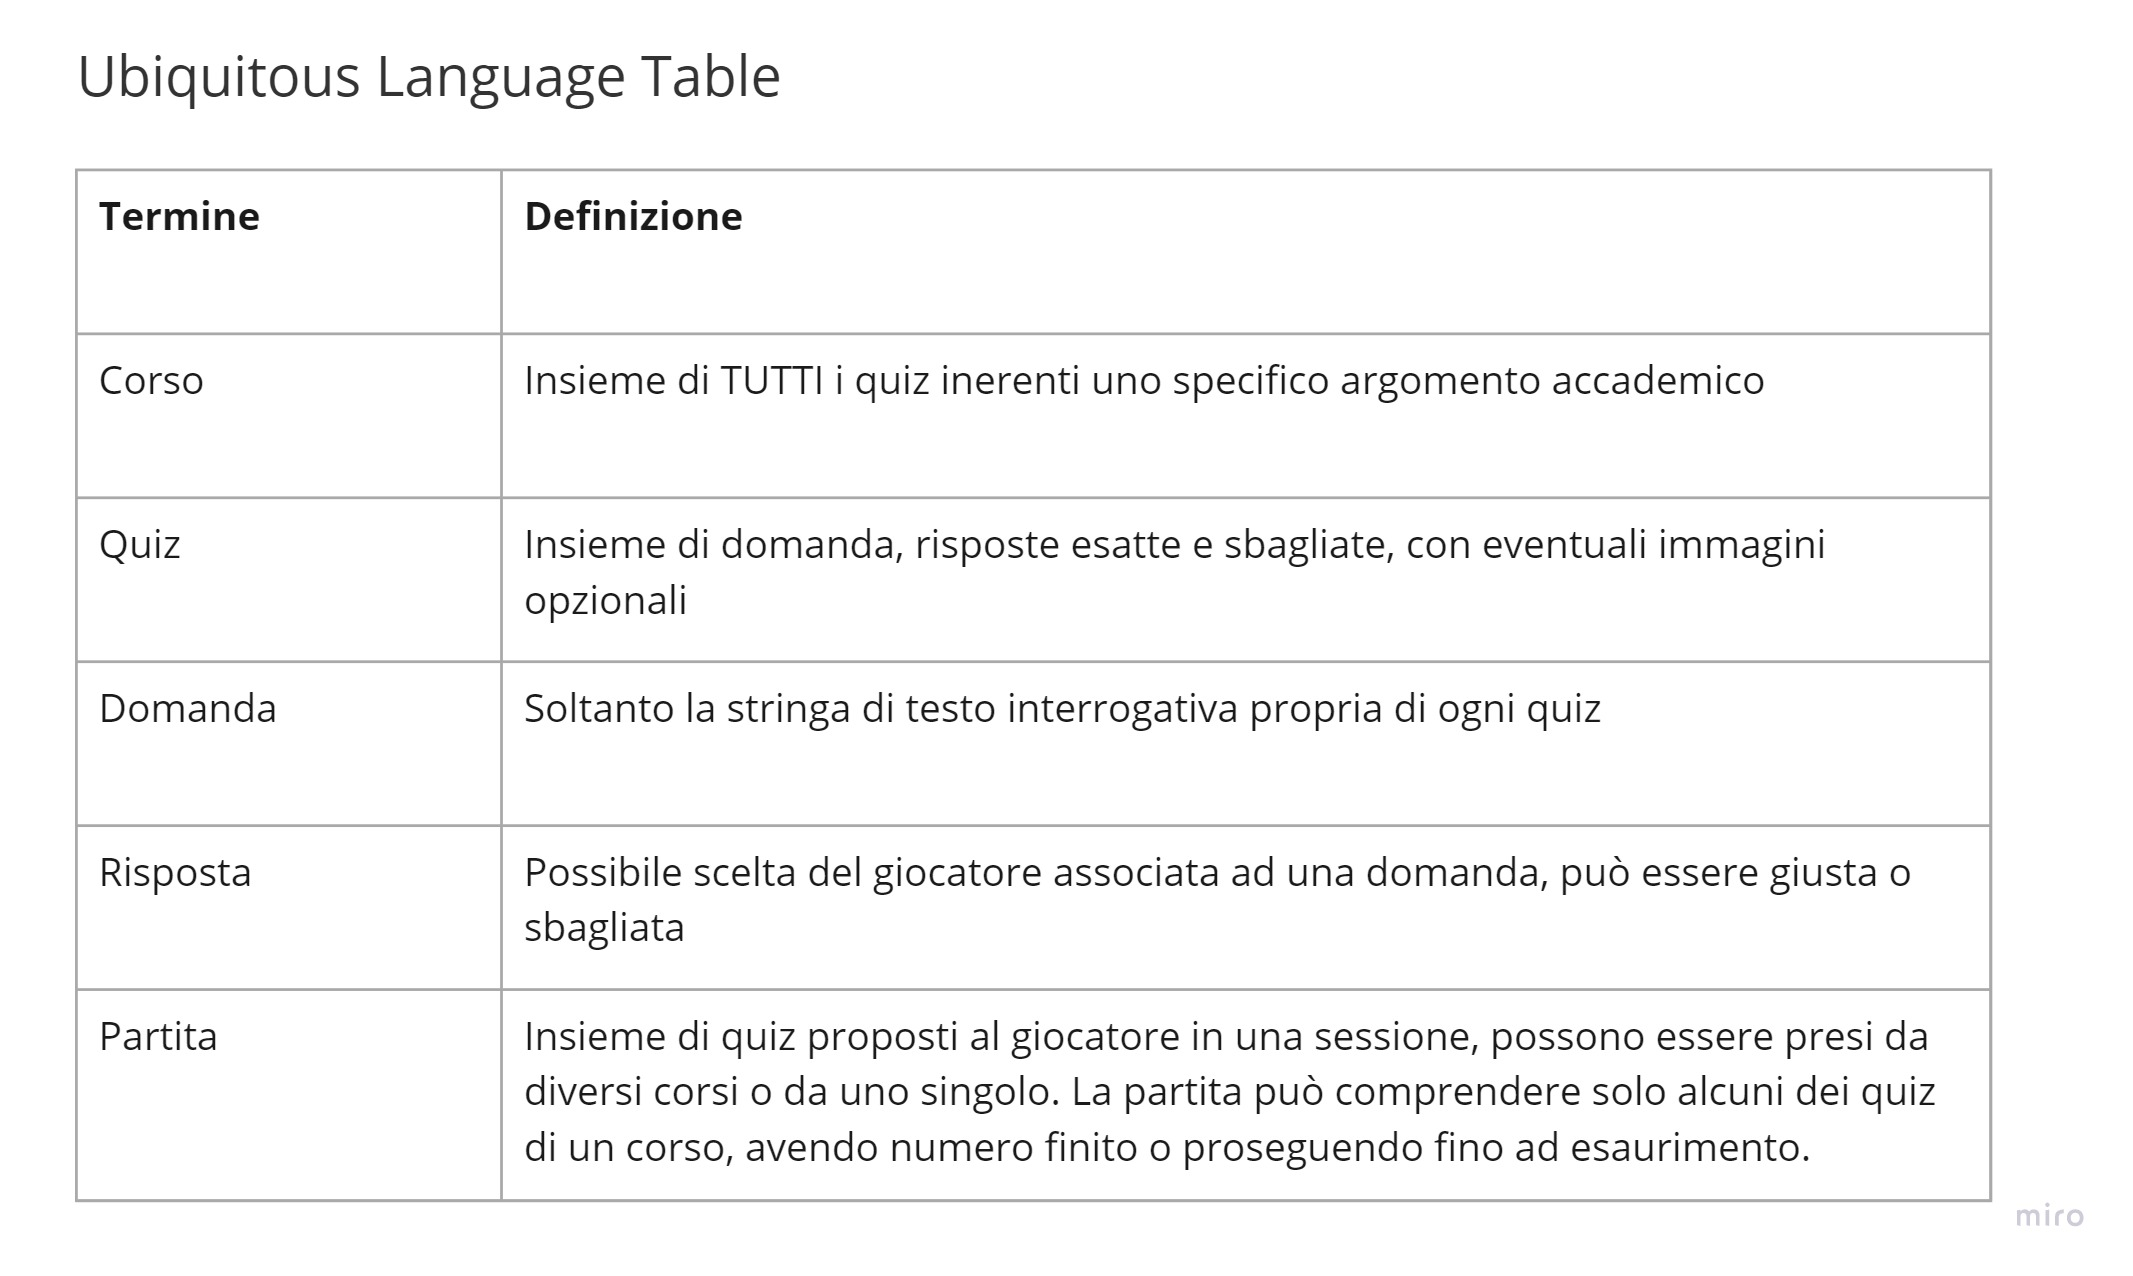
\includegraphics[width=0.9\textwidth]{Miro/ubiquitous-language.jpg}
        \caption{Tabella ubiquitous language}
        \label{fig:ubiquitouslanguage}
    \end{figure}